%\TEX root = ../../thesis_rui_almeida.tex
\section{DOAS Tomography}%
\label{sec:doas_tomography}

\todo[inline]{The structure of the thesis has changed and this section
must be rewritten. The paper on DOAS tomography is not being included as
a part of the thesis document, and therefore we may report on it at our
own will. It will be included in the end as separate document appendix.}

Measurement results from \gls{DOAS} experiments are line integrals. They
describe the number of molecules that is traversed by light in a given
direction (the direction towards which the instrument is pointing).
Thus, we can consider an experiment in which many of these instruments
are covering a given geographic region of the atmosphere in either 2 or
3 dimensions. This is a tomographic inversion problem, with the
projections being the \gls{DOAS} measurements.

Atmospheric spectroscopy as the data generating part of a tomographic
problem was first addressed in ~\todo{citation Shepp 1979}. In this
paper, the authors propose a computerised method employing a tunable
laser  and a set of mirrors for the retrieval of concentration values in
a two-dimensional circular region. Although not specifically concerning
\gls{DOAS}, the article established the basis for the technique.  The
most significant work corpus regarding DOAS Tomography came about only
in the 21\textsuperscript{st} century, when a group in the University of
Heidelberg dedicated themselves to determining two-dimensional trace-gas
concentration variations over a busy motorway in Germany - the BABII
campaign. 

During the course of this PhD, and as a credit requirement, I attended
several courses, namely in the Computer Science Department. One of them,
entitled "\emph{Advanced Software Development}" had as final requirement
the writing of a \gls{sms} on a topic of my choosing. This course
happened around the time I was starting to develop a \gls{DOAS}
tomography system, and one of the requirements of that work was to study
the state of the art to get a clear notion of how these systems were
being applied and developed globally. Therefore, this was the topic that
I chose for my \gls{sms}. The article (currently awaiting acceptance for
publication) is transcribed in full in Appendix~\ref{ap:tomDoas},  but I
include a selection of the most important parts in this section.

An \gls{sms} is a systematic first approach to a subject, and are
normally designed to retrieve a broad view of a given research area and
quantify the amount of evidence that there is in that specific field.
They share some similarities with \gls{slr} but work with much broader
data extraction and analysis procedures.Many times, they are used as
guides for primary research~\cite{Kitchenham2007}. In our case, the goal
was to understand the literary landscape of \gls{DOAS} tomographic
applications.

Figure~\ref{fig:sms_planning} denotes the whole process of conducting
an \gls{sms}. In general, \acrlong{sms} are comprised of 3 stages:
planning, conduction and reporting. The first stage is where the study
itself is parametrized. This stage does not directly represent any kind
of practical application, but it conditions and defines how the other
two stages will take place, and is probably the most important stage.

\begin{figure}[htpb]
    \centering
    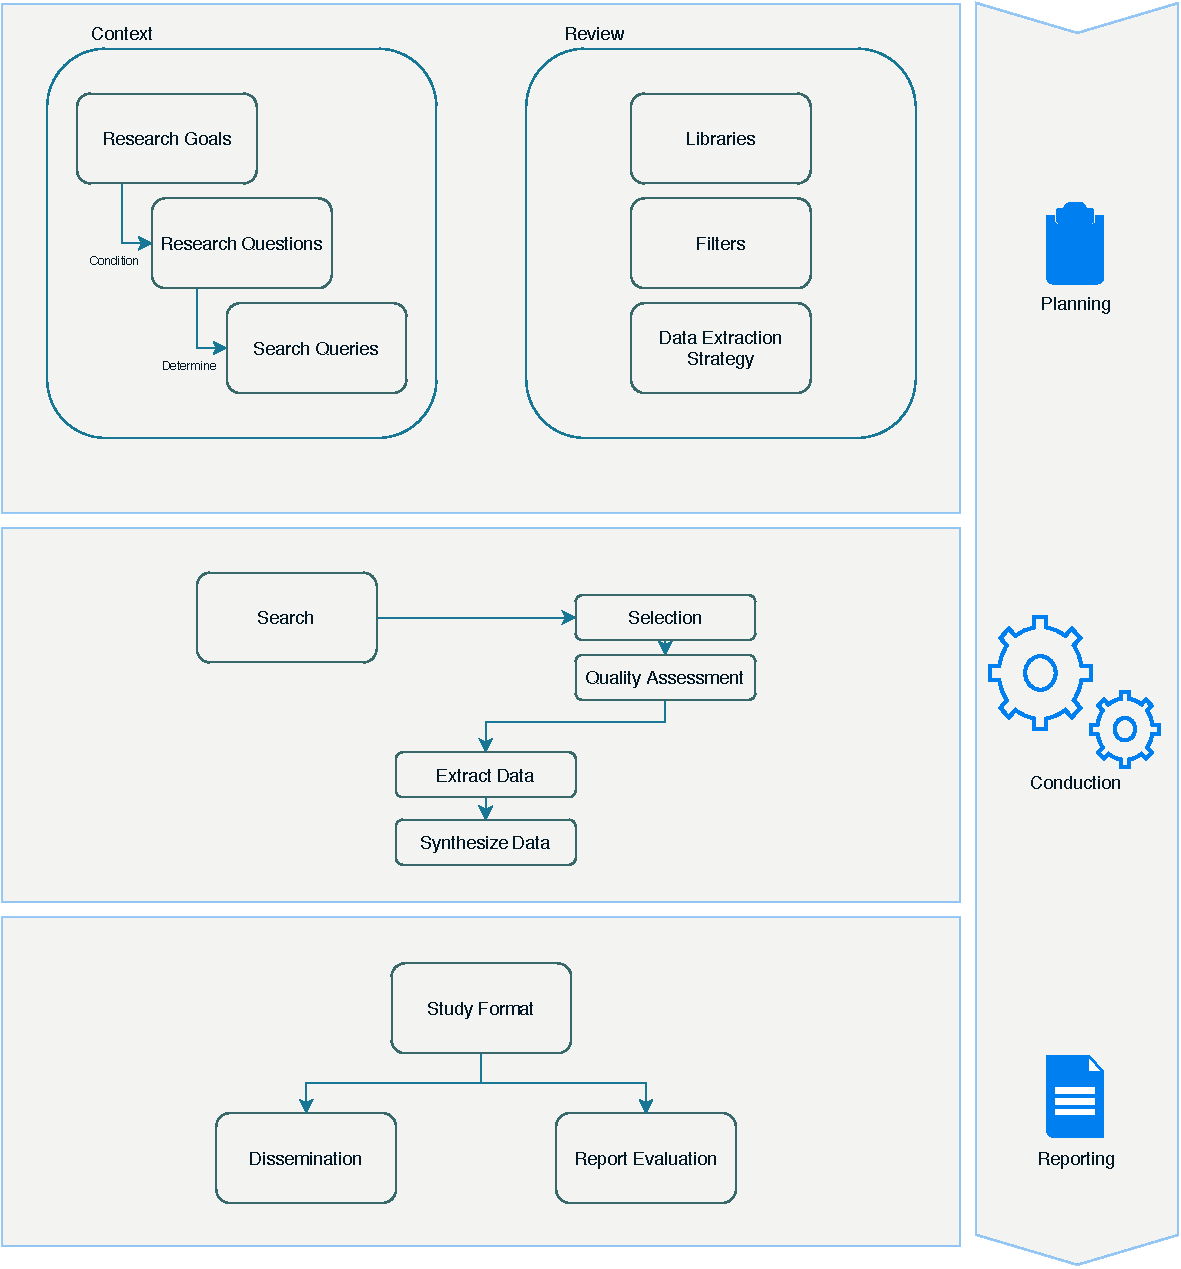
\includegraphics[width=.8\textwidth]{img/pdf/sms_planning.pdf}
    \caption{A schematic representation of an \gls{sms} writing process.
    The whole procedure is comprised of three smaller stages, which in
    turn are divided into various even smaller parts. The large arrow on the
    right represents the general evolution direction, although there is no
    rigid structure, and some back and forth is allowed and even expected.}
    \label{fig:sms_planning}
\end{figure}

There are two main components to the planning stage: the context and the
review. Broadly, these could be understood to define (respectively) how
the topics are to be searched and what it is that the authors are
looking for.

The context definition of the planning stage is when the authors define
the research questions and decide on the search protocol. The research
questions are defined according to the research goal, which in this case
was to assess the current status of the technology used in tomographic
\gls{DOAS}. A very common method for structuring the study's efforts is
the \gls{picoc} method. In our own case, this method is reflected in
Table~\ref{tab:picoc_sms}. The \gls{picoc} process rendered the original
research question, but it was not sufficiently specific in order to
conduct the search on. Therefore, we have sectioned the question into
three smaller and more manageable questions. The several questions are
detailed in Table~\ref{tab:sec_RQ}.

\begin{table}[htb]
\small
\centering
\caption{PICOC analysis.}
\label{tab:picoc_sms}
\begin{tabular}{@{}ll@{}}
\toprule
\textbf{Population} & DOAS research in general.\\
\textbf{Intervention} & The papers must address tomographic DOAS.\\
\textbf{Outcome} & Status \textbf{assessment} for \textbf{DOAS tomography}.\\
\textbf{Context} & Research papers.\\\bottomrule
\end{tabular}
\end{table}

\begin{table}[htb]
\centering
\small
\caption{Research question slicing}
\label{tab:rq_slicing}
    \begin{tabularx}{\textwidth}{lX}
        \toprule
        \textbf{Original} & What is the current status of the technology used in
        tomographic DOAS? \\
        \textbf{RQ1} & Is there a typical hardware setup used in tomographic
        DOAS studies? \\
        \textbf{RQ2} & Is there a standard software used to perform these
        analysis? \\
        \textbf{RQ3} & What are the algorithms more commonly used?\\\bottomrule
    \end{tabularx}
\end{table}

The review step of the planning stage starts by the definition of the
search queries and the electronic libraries in which they would be
searched.  Preliminary searches indicated that, although the topic was
well-established as a measuring technique, literature on the subject was
not widely available. Therefore, the search query was intentionally
vague: \textbf{DOAS atmospher* tomography}, with the asterisk working as
a wild card. As to the electronic libraries, and from the same
preliminary searches, we understood that the search would have to
involve the broadest repositories available. After experimenting a
little further, we decided to base our study in the libraries presented
in Table~\ref{tab:libraries_sms}.

\begin{table}[htb]
\centering
\caption{Electronic libraries used in this study.}
\label{tab:libraries}
    \begin{tabularx}{\textwidth}{ll}
        \toprule
        \textbf{Library}          & \textbf{URL}\\
        \midrule
        Google Scholar (GS)   & https://scholar.google.com/\\
        Web of Knowledge (WoK)& https://webofknowledge.com\\
        Scopus (SD)   & https://www.scopus.com\\
        % IEEE             & http://ieeexplore.ieee.org/\\
        % AGU Publications (AGU) & http://agupubs.onlinelibrary.wiley.com/hub/\\
        \bottomrule
    \end{tabularx}
\end{table}

Exclusion and inclusion filters are what determines what papers are kept
from those that are originally found by the search process and are
therefore important parameters of an \gls{sms} study.
Table~\ref{tab:inx_exc_criteria} provides a list of the filters that were
used in our study. To a certain degree, the application of these filters
are the first step of the data extraction process. Their definition is
thus part of the data extraction strategy, which determines the
guidelines with which the authors are to retrieve the target information
from the resulting literary corpus.

\begin{table}[htb]
\centering
\caption{Selection filters in use for this study's search.}
\label{tab:inx_exc_criteria}
\begin{tabularx}{\textwidth}{lXl}%{@{}cll@{}}
\toprule
\multicolumn{1}{l}{} & \textbf{Criterium} & \textbf{Definition} \\ \midrule
\multirow{1}{*}{\textbf{Exc. Criteria}} & EC1 & Satellite data papers
are not accepted \\
\midrule
\multicolumn{1}{l}{\multirow{3}{*}{\textbf{Inc. Criteria}}} & IC1 &
Results must be journal papers \\
\multicolumn{1}{l}{} & IC2 & Results must be about Tomographic DOAS \\ 
\multicolumn{1}{l}{} & IC3 & Results must be written in English \\
\bottomrule
\end{tabularx}
\end{table}

One of the most important parts of the data extraction strategy is how
to evaluate each paper with respect to its quality. For this study, and
although this is anything but an objectively defined topic, evaluation
was performed according to the formula in
Equation~\ref{eq:qual_formula}, where $Q_i$ is the paper's quartile and
$C_i$ is the number of citations that each particular study has gathered
throughout the years, which are represented by $Age_i$. In this
equation, $S$ represents the final quality score.

\begin{equation}
    \label{eq:qual_formula}
    S = Q_{i} \cdot \frac{C_i}{Age_i}
\end{equation}

While being a good indication on how the study will be conducted, the
presented method is not sufficiently specific for direct application.
Before proceeding, the research question is sliced according to the
\gls{picoc} analysis, resulting in what is presented through
Table~\ref{tab:rq_slicing_sms}.

\begin{table}[htb]
\centering
\small
\caption{Research question slicing}
\label{tab:rq_slicing_sms}
    \begin{tabularx}{\textwidth}{lX}
        \toprule
        \textbf{Original} & What is the current status of the technology used in
        tomographic DOAS? \\
        \textbf{RQ1} & Is there a typical hardware setup used in tomographic
        DOAS studies? \\
        \textbf{RQ2} & Is there a standard software used to perform these
        analysis? \\
        \textbf{RQ3} & What are the algorithms more commonly used?\\\bottomrule
    \end{tabularx}
\end{table}

The next step in this planning stage was to define the search queries
and the electronic libraries in which they would be searched.
Preliminary searches indicated that, although the topic was
well-established as a measuring technique, literature on the subject was
not widely available. Therefore, the search query was intentionally
vague: \textbf{DOAS atmospher* tomography}, with the asterisk working as
a wild card. As to the electronic libraries, and from the same
preliminary searches, we understood that the search would have to
involve the broadest repositories available. After experimenting a
little further, we decided to base our study in the libraries presented
in Table~\ref{tab:libraries_sms}.

\begin{table}[htb]
\centering
\caption{Electronic libraries used in this study.}
\label{tab:libraries_sms}
    \begin{tabularx}{\textwidth}{ll}
        \toprule
        \textbf{Library}          & \textbf{URL}\\
        \midrule
        Google Scholar (GS)   & https://scholar.google.com/\\
        Web of Knowledge (WoK)& https://webofknowledge.com\\
        Scopus (SD)   & https://www.scopus.com\\
        % IEEE             & http://ieeexplore.ieee.org/\\
        % AGU Publications (AGU) & http://agupubs.onlinelibrary.wiley.com/hub/\\
        \bottomrule
    \end{tabularx}
\end{table}

In the planning stage of the \gls{sms} it is also necessary to determine
the study's exclusion and inclusion criteria for found papers. Ours was
not an exception and these filters are presented in
Table~\ref{tab:select_filters_sms}.

\begin{table}[htb]
\centering
\caption{Selection filters in use for this study's search.}
\label{tab:select_filters_sms}
\begin{tabularx}{\textwidth}{lXl}%{@{}cll@{}}
\toprule
\multicolumn{1}{l}{} & \textbf{Criterium} & \textbf{Definition} \\ \midrule
\multirow{1}{*}{\textbf{Exc. Criteria}} & EC1 & Satellite data papers
are not accepted \\
\midrule
\multicolumn{1}{l}{\multirow{3}{*}{\textbf{Inc. Criteria}}} & IC1 &
Results must be journal papers \\
\multicolumn{1}{l}{} & IC2 & Results must be about Tomographic DOAS \\ 
\multicolumn{1}{l}{} & IC3 & Results must be written in English \\
\bottomrule
\end{tabularx}
\end{table}
